\begin{figure}[H]
  \centering
  \caption{Transition Maps (Variance Shock)}
  \begin{minipage}[t]{0.4\textwidth}
    \centering
    \small{(a) $\Delta$ Mean Welfare (CE)}
    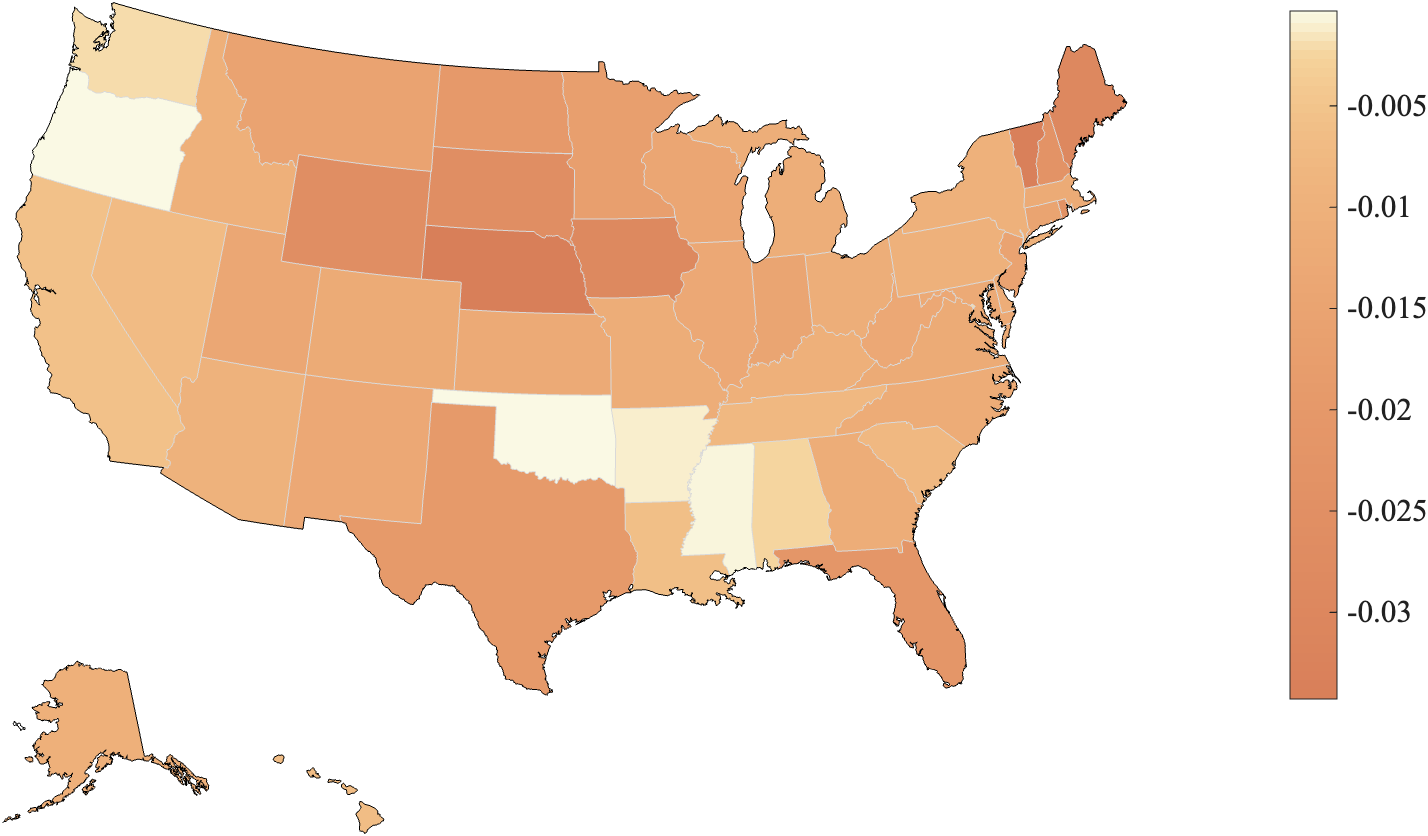
\includegraphics[width=\textwidth]{../Output/big_nu/graph_uncertainty_variance_shocks/transition_maps/transition_maps_delta_mean_welfare_ce.png}
  \end{minipage}\hfill
  \begin{minipage}[t]{0.4\textwidth}
    \centering
    \small{(b) $\Delta$ W/Y Ratio in level}
    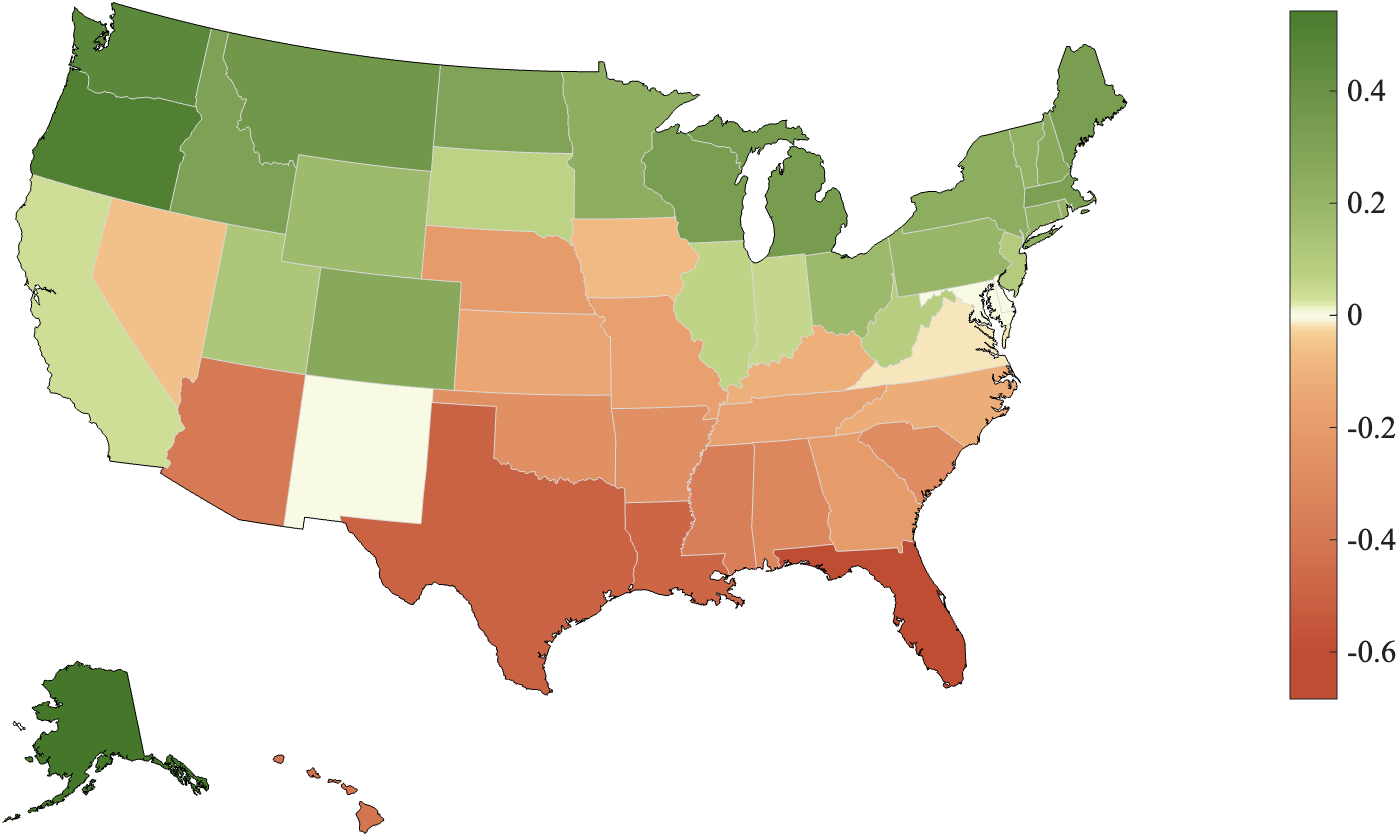
\includegraphics[width=\textwidth]{../Output/big_nu/graph_uncertainty_variance_shocks/transition_maps/transition_maps_wealth_income_ratio_changes.png}
  \end{minipage}\\[2ex]
  \begin{minipage}[t]{0.4\textwidth}
    \centering
    \small{(c) $\Delta$ Local Population (\%)}
    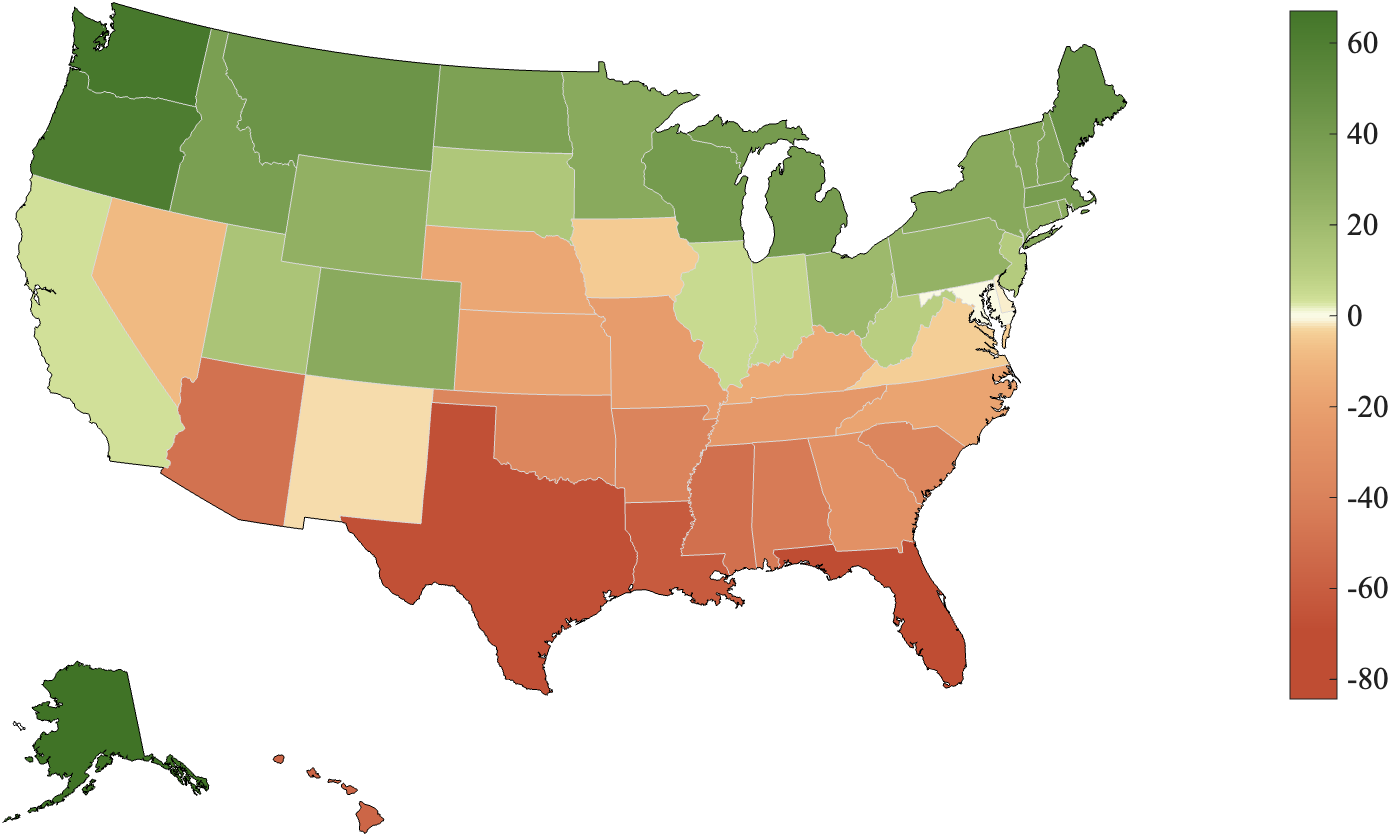
\includegraphics[width=\textwidth]{../Output/big_nu/graph_uncertainty_variance_shocks/transition_maps/transition_maps_local_pop_changes_pct.png}
  \end{minipage}\hfill
  \begin{minipage}[t]{0.4\textwidth}
    \centering
    \small{(d) $\Delta$ Mean Wealth (\%)}
    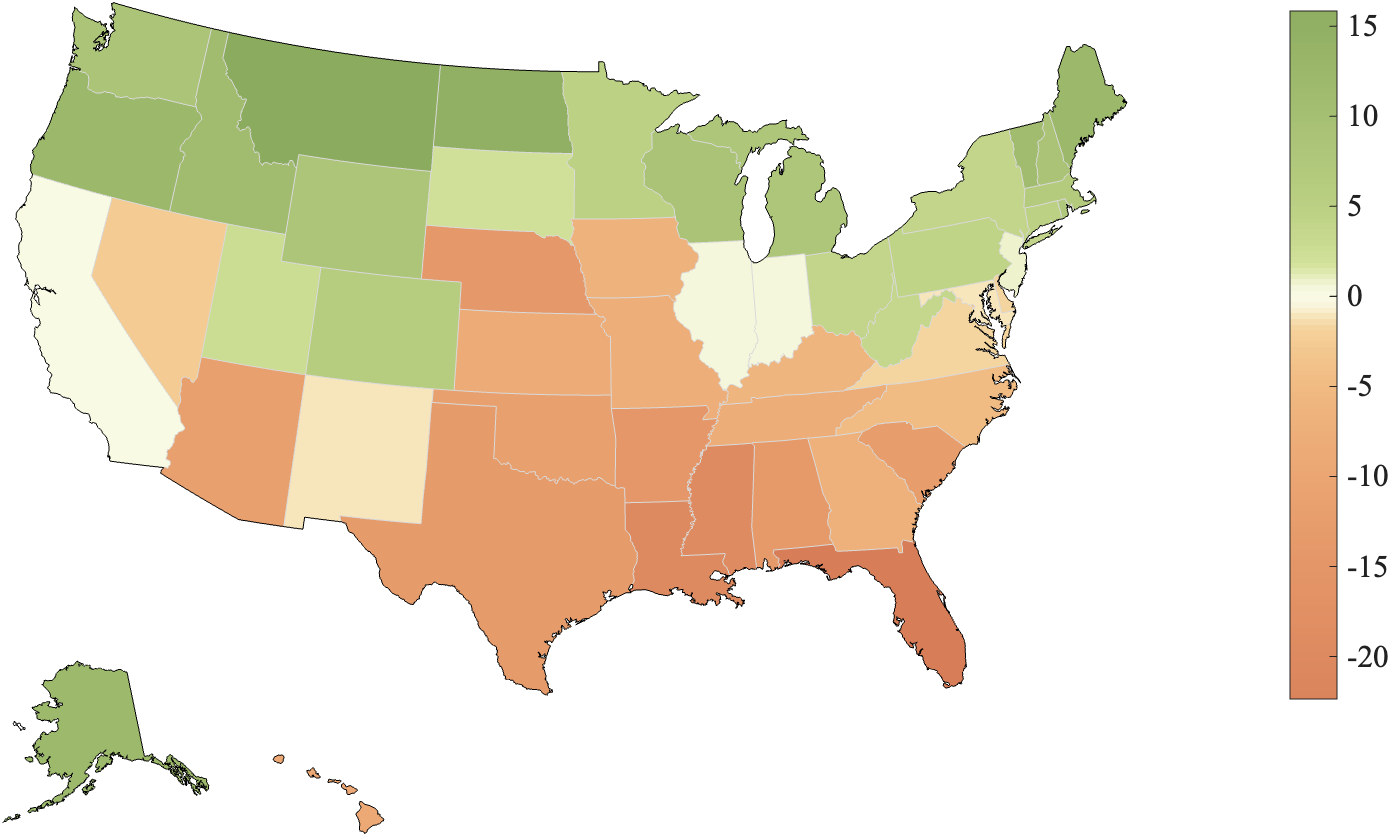
\includegraphics[width=\textwidth]{../Output/big_nu/graph_uncertainty_variance_shocks/transition_maps/transition_maps_pop_changes_pp.png}
  \end{minipage}
   \begin{minipage}{\textwidth}
  \vspace{0.5em}
  \footnotesize{\textbf{Note:} Spatial maps comparing the terminal steady state under 2100 climate parameters ($SS_\text{term}$) to the initial 2010 baseline steady state ($SS_\text{init}$) when introducing climate change variance-induced uncertainty. Panel (a): change in mean Certainty Equivalent welfare. Panel (b): change in state wealth-to-earnings ratio. Panel (c): relative population percentage change. Panel (d): percentage change in state mean per-capita wealth $\Delta \bar{a}_\ell\%$.} \end{minipage}
\end{figure}